\section{LEDs, ICs and headers}


		
		\begin{figure}[htbp!]
			\centering
			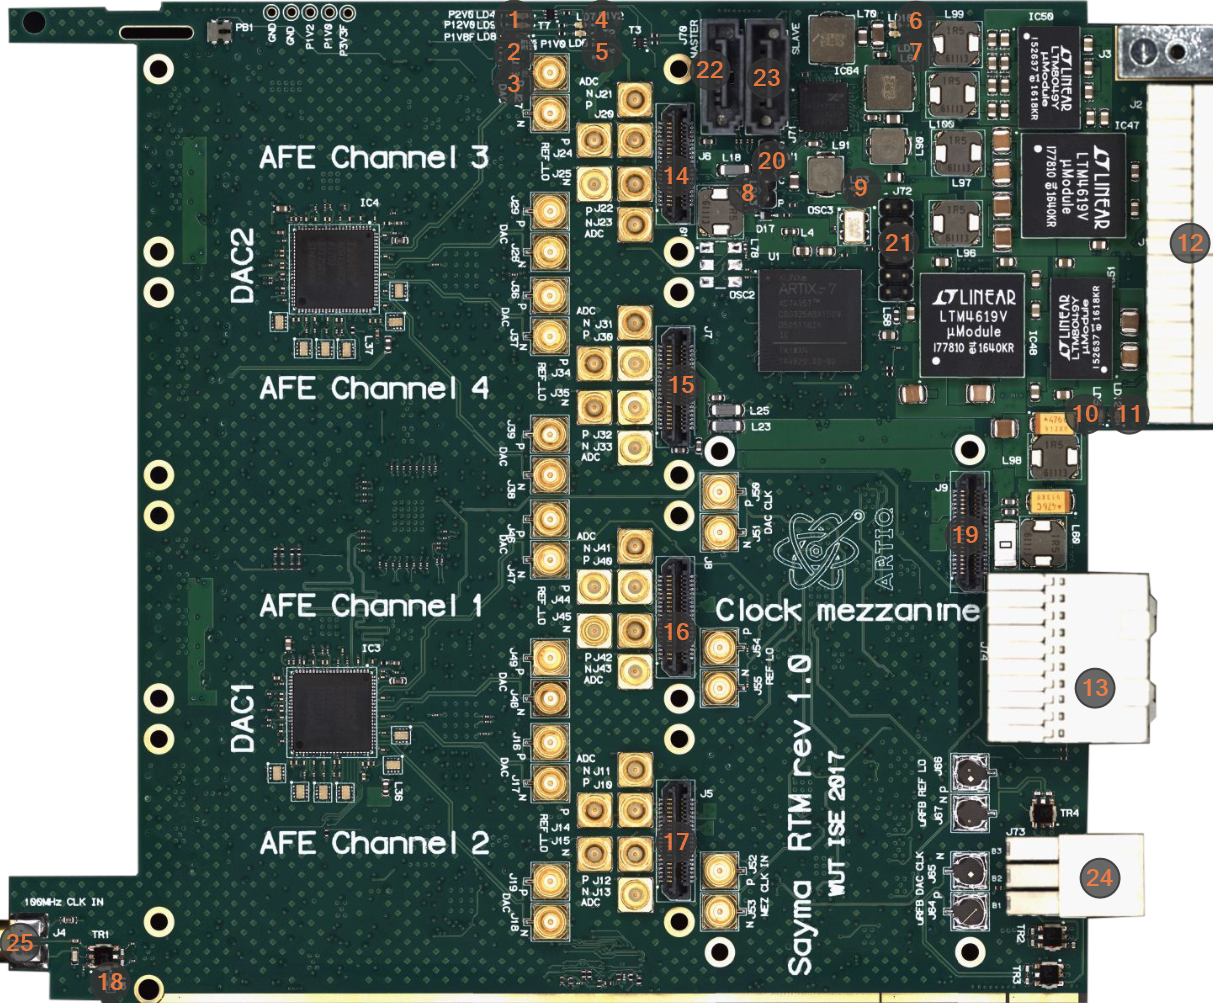
\includegraphics[width=12cm]{img/CalloutTop.png}\\
			\caption{Top view}
		\end{figure}
		
		\begin{figure}[htbp!]
			\centering
			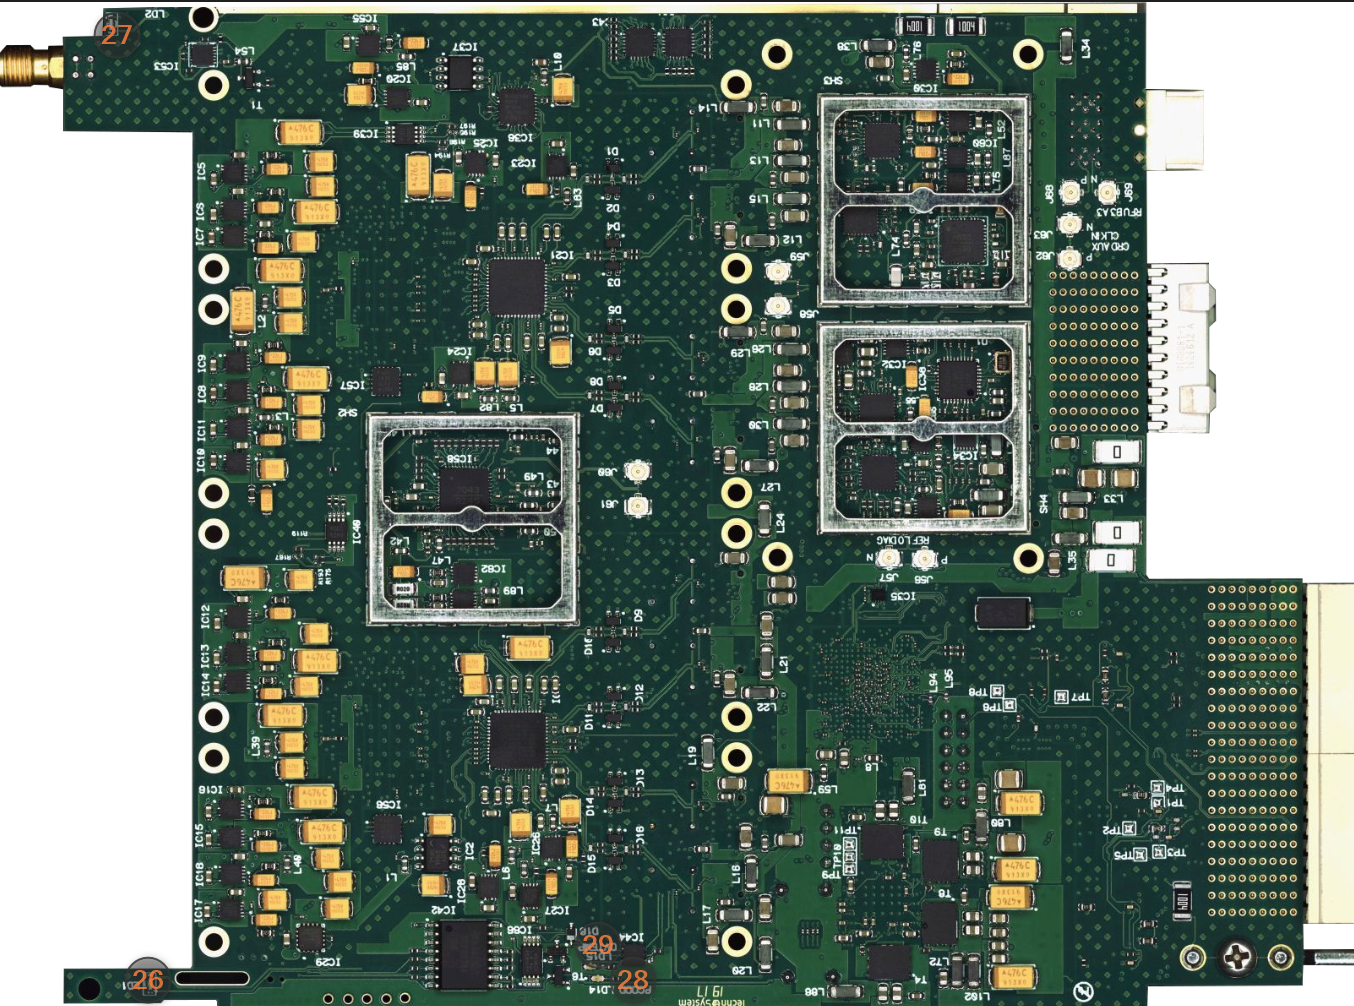
\includegraphics[width=12cm]{img/CalloutBot.png}\\
			\caption{Bottom view}
		\end{figure}
\clearpage

\begin{longtable}{|c|c|c|} \hline
	\multicolumn{3}{|c|}{Call out table } \\ \hline	
	Call out & Designator & Description \\ \hline
	12 & J2 & RTM Connector \\ \hline
	13 & J74 & uRFB Connector \\ \hline
	14 & J76 & Mezzanine 1 Connector \\ \hline
	15 & J76 & Mezzanine 2 Connector \\ \hline
	16 & J76 & Mezzanine 3 Connector \\ \hline
	17 & J76 & Mezzanine 4 Connector \\ \hline	
	19 & J9 & CLK Mezzanine Connector\\ \hline
	20 & W1 & EXAR I2C header \\ \hline
	21 & J72 & Header with I/Os see Figure \ref{ios} \\ \hline
	22 & J70 & Master SATA  \\ \hline
	23 & J71 & Slave SATA \\ \hline
	24 & J73 & uRFB Conenctor \\ \hline
	25 & J4 & SMA, EXT 100 MHz input \\ \hline


\end{longtable}


Callout 18: U2 is
\begin{itemize}
	\item off if RTM is ok 
	\item red if RTM is in an error state
\end{itemize}

Callout 26: LD2 is
\begin{itemize}
	\item off if - user defined
	\item green if - user defined
\end{itemize}

Callout 27: LD1 is
\begin{itemize}
	\item off if RTM has initialized in crate
	\item blue if  power is cut off and is possible to remove the board
\end{itemize}

Callout 28: LD14 is
\begin{itemize}
	\item off if there is a problem with power converters
	\item green if all power chips send Power Good
\end{itemize}

Callout 25: LD15 is
\begin{itemize}
	\item off if RTM is ok
	\item green if RTM reach 80 degrees (power is cut off)
	\end{itemize}


\begin{longtable}{|c|c|c|c|c|c|c|} \hline
		\multicolumn{7}{|c|}{Power LED table }\\ \hline
	Call out & Designator & Description&  Colour &nominal state& IC &Failure\\ \hline
	1 & LD4 & P2V0 & Green & on & Power & off \\ \hline
	2 & LD9 & P12V0 & Green & on & Power & off \\ \hline 
	3 & LD8 & P1V8 & Green & on & Power & off \\ \hline 
	4 & LD7 & P1V2 & Green & on & Power & off \\ \hline 
	5 & LD6 & P1V0 & Green & on & Power & off \\ \hline 
	6 & LD16 & P12V0A & Green & on & Power & off \\ \hline 
	7 & LD10 & N12V0A & Green & on & Power & off \\ \hline 
	8 & LD17 & P3V3 & Green & on & Power & off \\ \hline 
	9 & LD3 & P4V0 & Green & on & Power & off \\ \hline 
	10 & LD5 & P6V0A & Green & on & Power & off \\ \hline  	
	11 & LD12 & N6V0A & Green & on & Power & off \\ \hline  		 
\end{longtable}

\subsection{Headers pinout}

		\begin{figure}[htbp!]
			\centering
			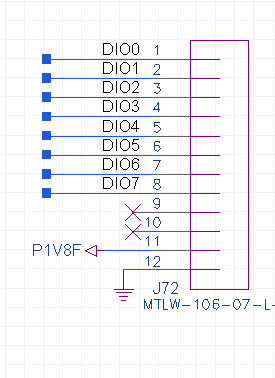
\includegraphics[width=8cm]{img/io.png}\\
			\caption{DIO - Call out 21} \label{ios}
		\end{figure}
%
%		\begin{figure}[htbp!]
%			\centering
%			\includegraphics[width=9cm]{img/jtaglpc.png}\\
%			\caption{JTAG - Call out  21}
%		\end{figure}
%		
%		\begin{figure}[htbp!]
%			\centering
%			\includegraphics[width=9cm]{img/gpio.png}\\
%			\caption{DIO - Call out 23}
%		\end{figure}

\clearpage


%\begin{longtable}{|c|c|c|} \hline
%		\multicolumn{3}{|c|}{Tespoints table}\\ \hline
%	TPx & Sig Name & LPC pin \\ \hline
%	TP1 & MII1\_col & C13 \\ \hline
%	TP2 & SDCLK & J10 \\ \hline
%	TP3 & SDCMD & K14 \\ \hline
%	TP4 & SDPWR & K11 \\ \hline
%	TP5 & SDDAT0 & L14 \\ \hline
%	TP6 & SDDAT1 & M12 \\ \hline
%	TP7 & SDDAT2 & N14 \\ \hline
%	TP8 & SDDAT3 & M11 \\ \hline
%	
%\end{longtable}	


\subsection{Location ICs}

		\begin{figure}[htbp!]
			\centering
			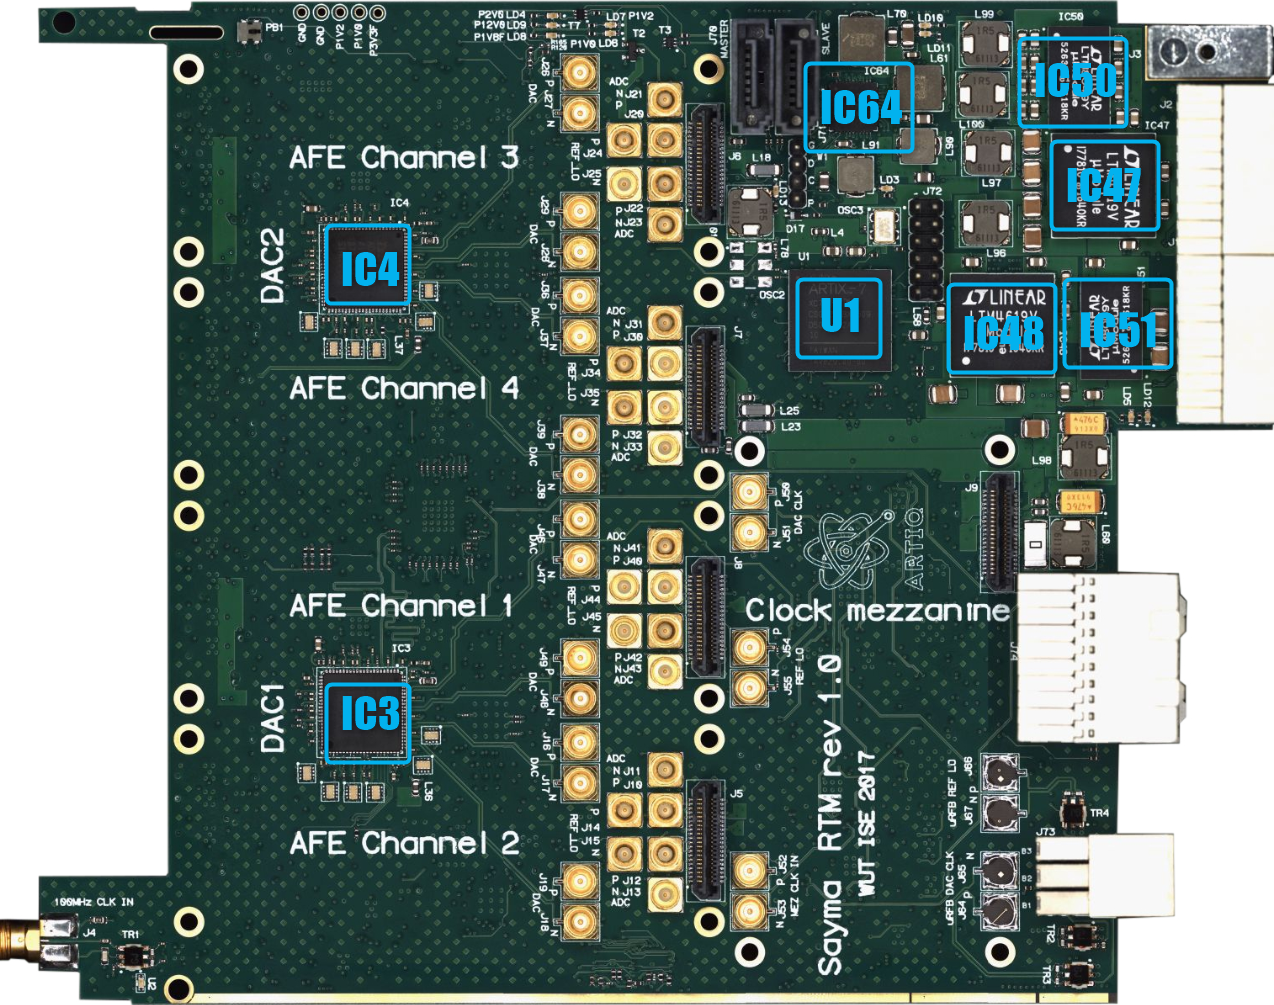
\includegraphics[width=12cm]{img/TU1.png}\\
			\caption{Top}
		\end{figure}
		\begin{figure}[htbp!]
			\centering
			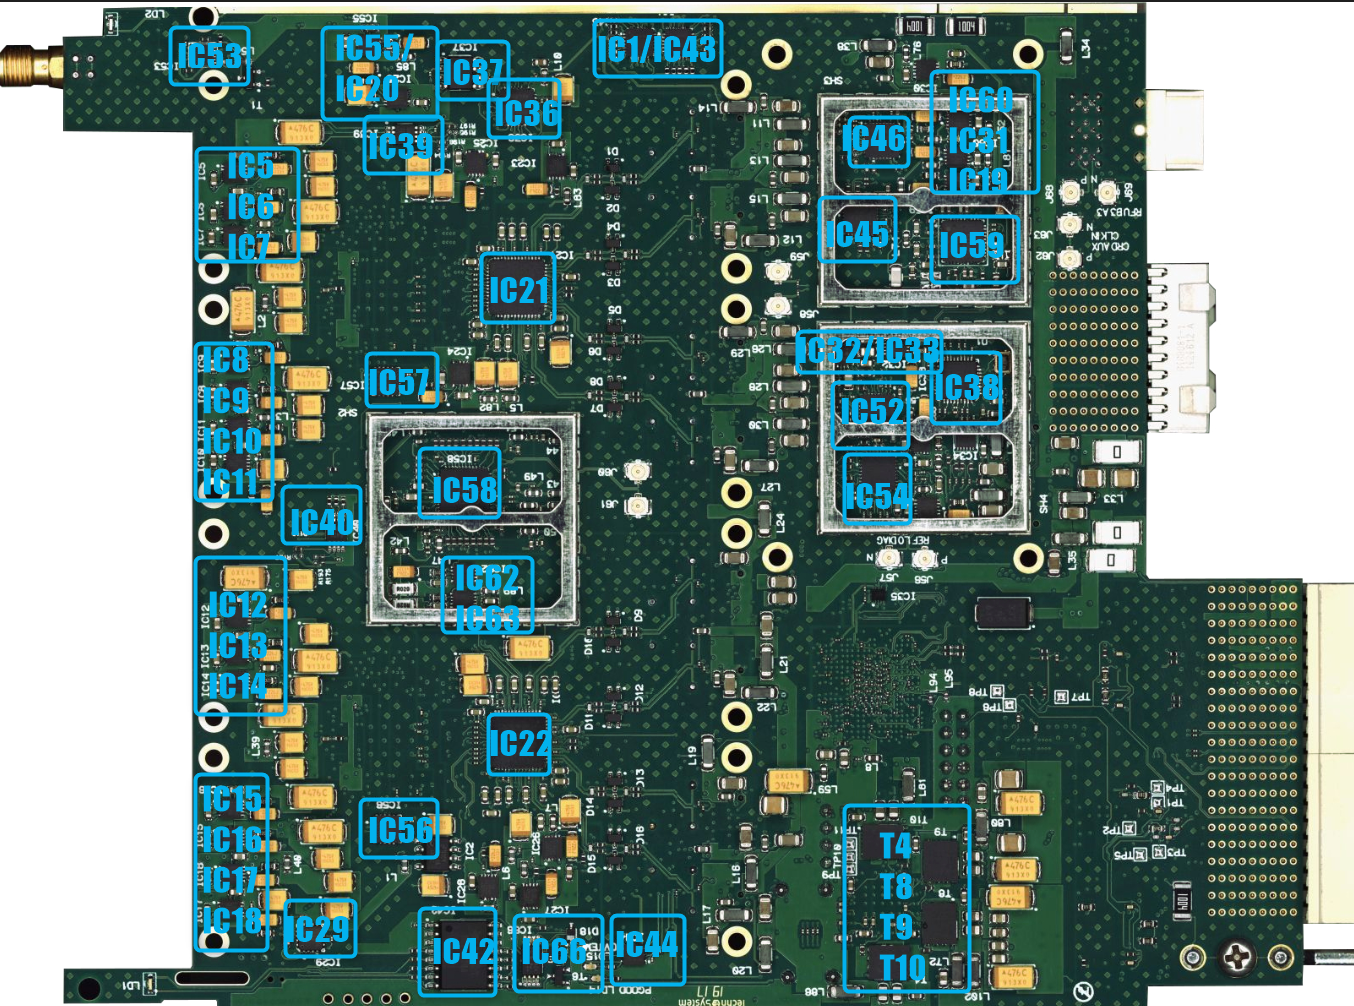
\includegraphics[width=12cm]{img/BU1.png}\\
			\caption{Bottom}
		\end{figure}
\clearpage

\begin{longtable}{|c|c|c|} \hline
		\multicolumn{3}{|c|}{ICs Location}\\ \hline	
	Ux & IC & Description \\ \hline
	U1 & Artix-7 & FPGA \\ \hline
	IC1/IC43	&	TCA9548		& I2C MUX 			\\	\hline	
	IC3 & AD9154 & DAC1 \\ \hline
	IC4 & AD9154  & DAC2\\ \hline
	IC5/IC6/IC7	&	LT3045		&  	DAC supply		\\	\hline
	IC8/IC9/IC10/IC11	&	LT3045		&  	DAC supply		\\	\hline	
	IC12/IC13/IC14 & LT3045 & DAC supply \\ \hline
	IC15/IC16/IC17/IC18 & LT3045 & DAC supply \\ \hline	
	IC20	&	LT3045		&  DAC supply			\\	\hline	
	IC21	&	AD9656		&  	ADC		\\	\hline
	IC22 & AD9656 & ADC \\ \hline
	IC29 & ADP1740 & P1V8 LDO \\ \hline	
	IC32 &	LT3045 & Si5324 power supply \\ \hline
	IC33 & ADM7151 & P5V0 LDO \\ \hline
	IC36	&	AD7194		& ADC 			\\	\hline
	IC37	&	ADR440		&  ADC reference			\\	\hline
	IC38 & Si5324 & Clock recovery \\ \hline	
	IC39 & LM75 & Temp sens \\ \hline
	IC40 & LM75 & Temp sens \\ \hline	
	IC42 & PCF8574 & I2C to GPIO extender \\ \hline	
	IC44 & MAX6642 & Temp sens \\ \hline
	IC45	&	ADCLK948		&  Clock buffer		\\	\hline
	IC46	&	ADCLK948		& Clock buffer 		\\	\hline					
	IC47 & LTM4619 & Buck converter P2V0 and P4V0\\ \hline
	IC48 & TPS 74401  & Buck converter P6V0\\ \hline
	IC50 &  LTM8049 & Buck converter P12V0A and N12V0A \\ \hline
	IC51 & LTM8049& Buck converter N6V0A \\ \hline
	IC52 & ADCLK948 & Clock buffer \\ \hline
	IC54 &ADCLK948 & Clock buffer \\ \hline	
	IC53	&	LTC6957		&  Isolation external clock input			\\	\hline	
	IC55	&	LT3045		&  DAC supply			\\	\hline	
	IC56 & ADT7420 & Temp sens \\ \hline
	IC57 & ADT7420 & Temp sens \\ \hline
	IC58	&	HMC7043		&  	Clock buffer		\\ \hline
	IC59	&	HMC830		&  	Clock buffer		\\	\hline
	IC62/IC63		& LT3045	& HMC7043 power supply	\\ \hline			
	IC64 & XR77129 & EXAR \\ \hline
	IC66 & AT24MAC402 & EEPROM \\ \hline
	T4/T8/T9/T10 & FDMS7608S & Exar transistors\\ \hline




																										
\end{longtable}



